\chapter{Software for experiment control and analysis}\label{chap:software}

[TODO: better screenshots: example.py? Monkeypatch to hide errors in BLACS?]

Software underlies a huge part of physicists work, whether experimental or theoretical. On the experimental side in our field, increasingly complex and precise experiments in atomic physics require increasingly sophisticated control of the lasers, magnetic coils, frequency synthesisers, cameras, etc that interact with the quantum systems we study. These devices necessitate an interface, between themselves and the experimentalist, and whilst the interfaces of the past were more likely to be knobs and dials on the front of the device, they are increasingly taking the form of software. Software is needed to convert from a smooth ramp of voltages designed to ramp up a magnetic field slowly into a finite list of voltages and times that a device can output with precise timing to make it happen. Software is needed to transmit this data to the device in question, in the format it requires. Software is required to extract the images and voltage traces from the cameras and voltage acquisition devices and store them in computer memory or on disk. And finally software is required to compute meaningful results from this raw data.

A large fraction of my time during my PhD was spent developing, maintaining and improving the laboratory control system software suite that has emerged from our group at Monash---the \emph{labscript suite}. Originally envisioned as a Python [CITE]library for generating arrays of hardware instructions to be programmed into devices via a LabVIEW VI [CITE? Registered trademark?] in a manner similar to most existing control systems in our field, the software suite grew to encompass most aspects of day-to-day control and analysis in our labs. At present it comprises about five separate programs/libraries, depending on how one chooses to draw the borders between them, that control every aspect of a cold atom physics experiment from setting parameters to analysing results.

An overview of the process is shown in Figure~\ref{fig:labscript_flowchart}.

In this (short) chapter, I'll first give a quick overview of each program and what it does. Then I'll outline the design and development approaches we have taken with the labscript suite and comment on the effects these choices have had on the course the project has taken over the last few years. Then I'll summarise recent developments since the publication of our paper on the software; \emph{A scripted control system for autonomous hardware-timed experiments}~\cite{starkey_scripted_2013}, which is reproduced at the end of this chapter. Further details on the role of each program in the suite and the design underlying it are available in the paper, and a more detailed presentation of the software, its design principles, and recent and future developments is available in Philip Starkey's thesis [CITE].

\begin{figure}
\begin{center}
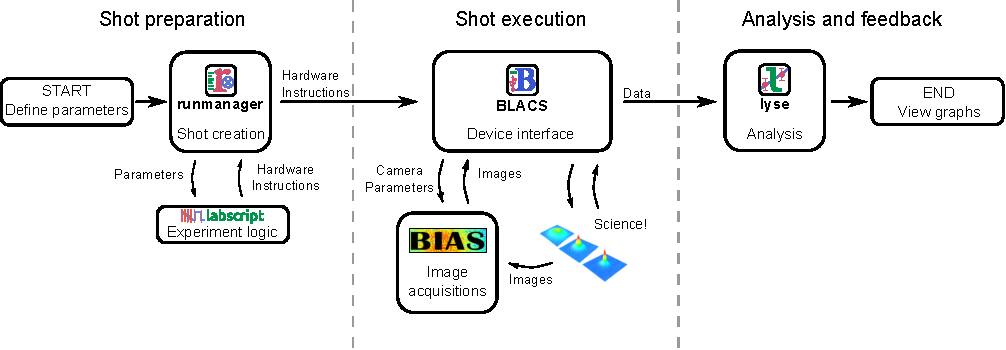
\includegraphics[width=\textwidth]{figures/software/flow_chart_simple-eps-converted-to.pdf}
\caption{The labscript suite comprises a number of libraries and programs allowing one to perform precisely timed experiments, each run of which we call a `shot', using commodity hardware such as devices from SpinCore, NovaTech, National Instruments and others. Experiment logic is described by the user in the form Python code using the \texttt{labscript} Python module, which produces from the user's code a set of low-level instructions appropriate for being programmed into the hardware. The program \texttt{runmanager} provides a graphical interface for inputting parameters into this experiment logic, and allows this process to be repeated to produce multiple sets of instructions for repeated execution of the experiment with different input parameters. Not shown in this flowchart is \texttt{runviewer}, which is a graphical program displaying plots of the instructions that have been generated by \texttt{labscript}. One the instrucitons have been generated, the program \texttt{BLACS} (Better Lab Apparatus Control System) is responsible for communicating with the hardware: programming in the generated instructions, beginning the experiment, and saving any acquired data to file. An auxiliary LabVIEW program called \texttt{BIAS} (BEC Image Acquisition System) is used for communication with cameras in Monash quantum fluids group laboratories, though other groups use a number of alternate programs in its place, including a stripped-down derivative of BIAS called unBIASed, as well as several Python-based `camera servers'. After BLACS is finished with a shot, the data is passed to \texttt{lyse}, which executes user-written analysis scripts on each shot to analyse the results, and also executes scripts that operate on sets of data over multiple shots, producing interactive plots. Runviewer provides a Python library for producing shots with programatically provided parameters, allowing the flowchart to close into a loop and produce shots based on analysis results. This has been used to optimise experiment outcomes with respect to a give figure of merit.}\label{fig:labscript_flowchart}
\end{center}
\end{figure}

\section{The programs}


\subsection{labscript}

Labscript isn't a program but rather a library: that is, it is a set of classes, functions and methods that can be called from user-written code. We call labscript a \emph{compiler}, because what the functions, classes and methods within it do is generate tables of low-level instructions appropriate for programming into devices to execute the experiment described by the user. Thus the user writes a line of code like \verb|MOT_beams.constant(t=3, 1, 'V')| and this will add an entry to the table of instructions for whichever DAC is controlling the MOT beams to go to three volts at $t = 3\unit{s}$ after the beginning of the experiment. This is a simple example, but has advantages over having a human write the table directly.\footnote{Most existing control systems in our field are more-or-less in the form of a large table with each row corresponding to a particular time in the experiment, with the user editing values in the table directly, or typing mathematical expressions in th table describing values as a function of time between one row of the table and the next.} After one has told the labscript compiler with this line that the MOT beams should have their control voltage set to three volts, it knows that at all later times the same state should remain, until the user says otherwise. Thus the user doesn't need to also change all future rows of the table: it it enough to declare a change. 

Labscript automates much of the tedious, repetitive work that is required in generating those lists of voltages, frequencies, and digital values required to control an experiment. This tedium mostly comes from the fact that devices are sharing timing (see the paper for a description of \emph{pseudoclocking}, the method by which the timing of devices is controlled). When one device changes state, several devices may receive a timing pulse at that time, and so they must have an entry in their corresponding tables in order to output the correct value (possibly the same as the previous value they were outputting) at that time, lest they get too far ahead and output a value that was meant for a later time. Labscript takes high level descriptions of what voltages etc.~are required at different times, puts them on a common timing base and generates the correct tables of values. It also collects any other instructions such as camera exposure durations, or the position a translation stage should move to at the start of the experiment even though it is not capable of moving quickly during the experiment. These instructions are processed by labscript and saved to a file in HDF5 format [CITE]. For more information, see the paper at the end of this chapter, and Philip Starkey's thesis [CITE CURRENTLY IN PREPARATION TO BE SUBMITTED].

\subsection{runmananger}

A thirty second or so experiment is not the only timescale on which experimentalists require automation. Ordinarily the same experiment is repeated over a range of input parameters, with several input parameters varying to span some parameter space. In addition there are many parameters involved in an experiment that do not vary often, but nonetheless need to be managed. Runmanager is a graphical program for entering and managing these parameters and describing the parameter spaces over which they should vary. Users can enter simple numbers into the interface (or other non-numerical variables), or lists of numbers that will be considered a description of a dimension of a parameter space. These dimensions may be combined in an outer product resulting in a larger space, or equal length dimensions may be looped over in tandem, if the two variables are intended to vary together rather than separately.

The graphical interface of runmanager is shown in~\figref{fig:runmanager}. Runmanager produces the initial HDF5 files that are passed to the user's labscript code, which the user writes in the form of a Python script that makes use of the labscript library. The user specifies in runmanager's interface which python file contains their `experiment script'. When the user clicks `engage', runmanager produces one HDF5 file---each containing a set of globals---for each point in the parameter space described by the globals currently selected in the runmanager interface. For each HDF5 file runmanager initialises the labscript library such that these values become global variables from the perspective of the users experiment script, which then runs. The labscript library then writes the resulting hardware instructions to that same HDF5 file.

We refer to the process of passing the HDF5 file to the user's code and running it as `compilation', and the resulting HDF5 file containing both globals and hardware instructions a `compiled shot file'. Compilation occurs in a separate process from the runmanager graphical interface, allowing a clean separation between user code and runmanager, so that even the most low-level crashes of the user's code cannot crash runmanager and only require a restart of its subprocess. This type of separation is a repeated occurrence in the labscript suite and has been invaluable for making robust programs that can keep operating in the case of inevitable crashes of user code, or of bugs within the labscript suite itself.

\begin{figure}
\begin{center}
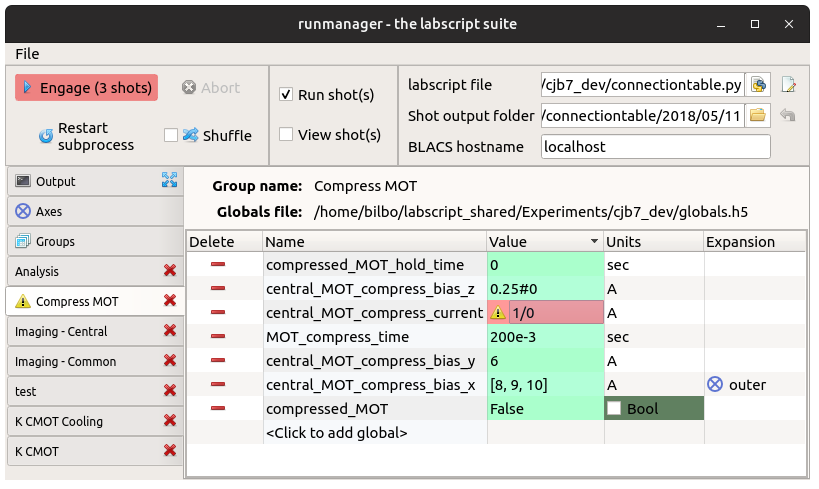
\includegraphics[width=\textwidth]{figures/software/new_screenshots/runmanager.png}
\caption{Runmanager as of 2018, showing the interface for entering `globals', so called because they appear to the user's code as global variables. Boolean globals can be turned on and off with a checkbox, and expressions resulting in an error are highlighted in red. The `expansion' column is how one chooses whether a global should be considered a list of values to loop over, re-running the experiment each time, and if so if that loop should be combined with other such globals to loop over the resulting product space (`outer') or whether the globals should be looped over together (`zip'). Zipped globals can be grouped together by typing a name in the expansion column to identify which `zip group' the global belongs to. Globals in the same zip group will loop together, and multiple zip groups will form separate axes of a product space.}\label{fig:runmanager}
\end{center}
\end{figure}

\subsection{runviewer}
[SCREENSHOT]

\subsection{BLACS}

\begin{figure}
\begin{center}
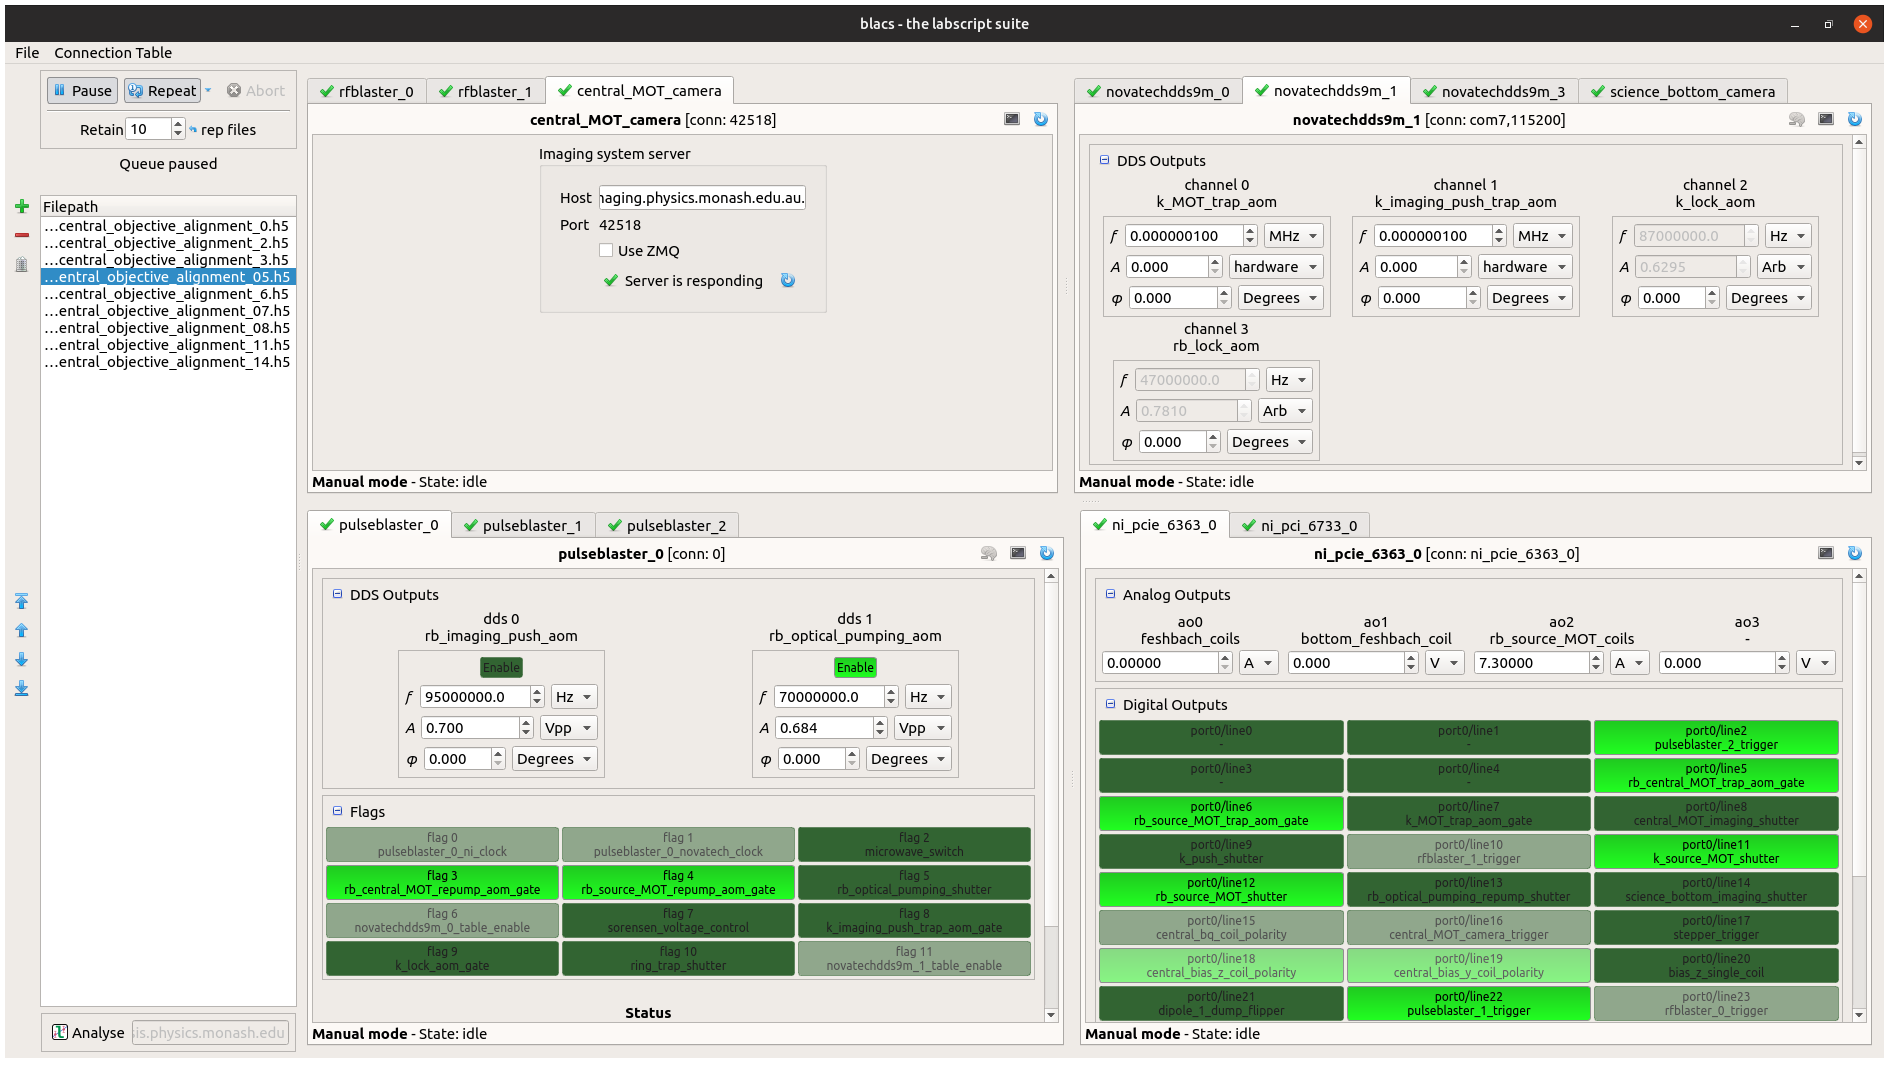
\includegraphics[width=\textwidth]{figures/software/new_screenshots/blacs.png}
\caption{BLACS as of 2018}\label{fig:blacs}
\end{center}
\end{figure}

BLACS (Better Lab Apparatus Control System) is a graphical program responsible for queueing experiment shots as compiled by labscript and runmanager, and executing them one after the other on the hardware. As such, BLACS interacts with a number of python classes that function as \emph{drivers} for each devices, containing code that uses the required software libraries, hardware drivers or communication protocols to communicate with the devices in the manner required by each one individually. BLACS executes the code for communicating with each device in a separate process in order to isolate them from each other, so that communication failures, software bugs or other failures that may occur in the interactions with one device will not stop BLACS from continuing to function in other respects. Errors are presented graphically and each device process may be restarted with the click of a button if something goes wrong. This is useful for both responding to unexpected failure, as well as for debugging during the development of the driver for a new device (or of new features for an existing device) being integrated with the labscript suite.

\subsection{lyse}
\begin{figure}
\begin{center}
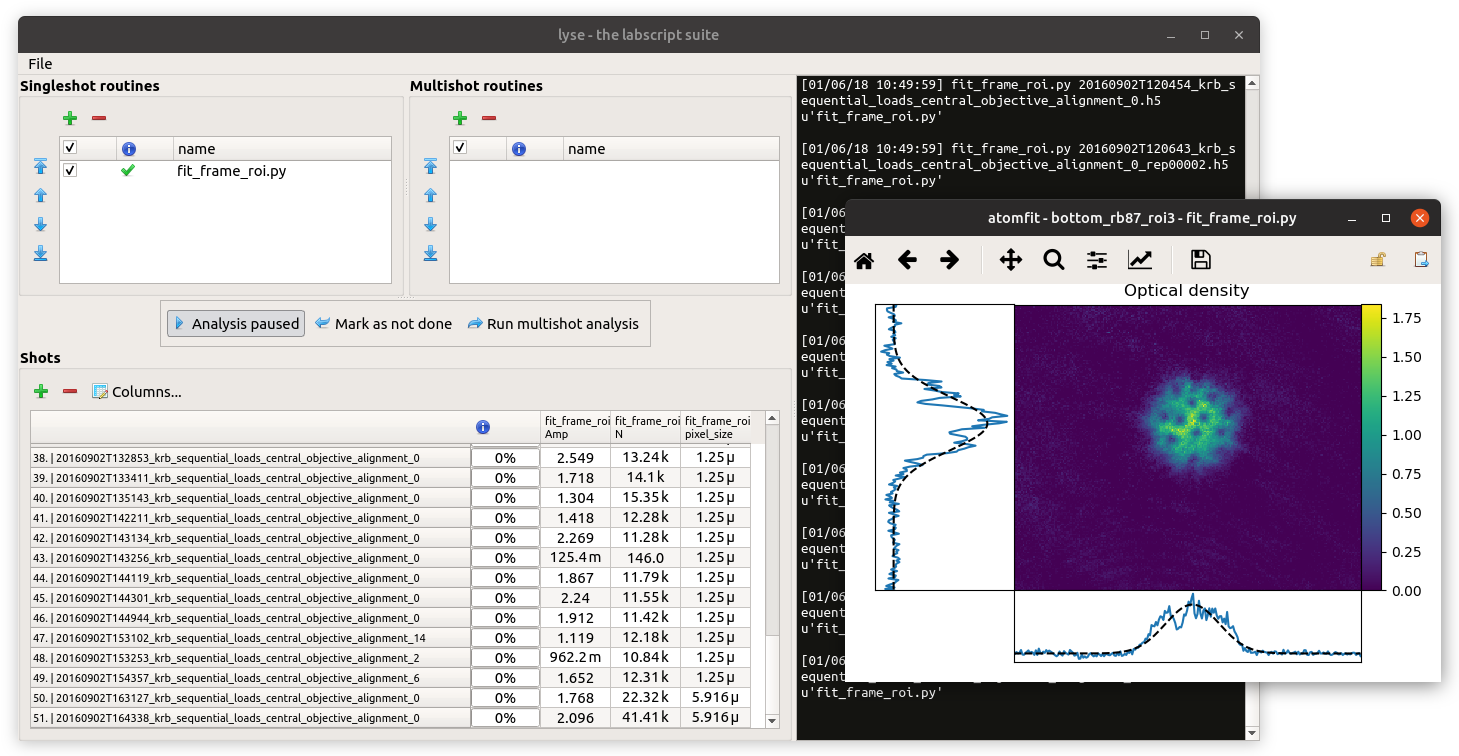
\includegraphics[width=\textwidth]{figures/software/new_screenshots/lyse.png}
\caption{Lyse as of 2018}\label{fig:lyse}
\end{center}
\end{figure}
[SCREENSHOT]

it's text:

standard tools

it's code: experiments are code.

unix philosophy:

disconnected parts with well defined interfaces easier to maintain. Easier to extend, people can put their own code in there.

open source and using open source libraries: advantage: patching upstream is a viable option. I have submitted and had patches accepted by numpy, pandas, h5py and pyzmq that improved their usability for specific use cases we have had. 

crowdsource bugfixes! Lots of competent programmers in physics groups. They implement long-standing features
that we have not had time to implement ourselves.

Popular, dynamic programming language
Allows us to hack on it to intoriduce custom behavour whilst keeping the benefits of using a general purpose programming language. Allows new students to get up to speed quickly. Allows interoperability with a wide range of tools and protocols for talking to other code and to hardware.

Standard format: HDF5


\section{Recent developments}
Firstly, far more people using the software.

Since the paper:

General:
A port to the Qt GUI toolkit, which occured while I was in the US visiting Ian. This toolkit is more widely used and cross-platform.
A proper installer such that installation is now running one script and works reliably across platforms.
An (almost complete) port to Python 3
Mise is no longer used, instead people are plugging lyse and the runamnager API into things like MLOOP. This demonstrates the pluggability of the system, but could be improved.
General polishing all round
More devices
Output capturing of subprocesses now captures ouput of subsequent subprocesses and extension code
More flexible camera interfaces, there are several Python camera servers. We no longer treat cameras as special, and if they need to be on a different computer for reasons of hardware or screen real estate, the remote devices feature will get that.
A port to the Qt GUI toolkit

Labscript:
Arbitrary function ramps
Markers
Inverted DO
Gated clocks: allow more devices to run off the same clock given very different memory capacities.

BLACS:
Repeat functionality repeat last
Delete repeated shots
Plugin mechanism
Optional Terminals visible for all devices for debugging purposes
Can be started without a Connection table
Bugfixes leading to faster times in between shots

runmanager:
Saving and loading of configuration settings
Finer control over parameter spaces: per-axis shuffle, control over axis loop order
Agnostic compilation: can be used to make parameter space scans for arbitrary things

runviewer:
Saving and loading of configuration settings
nonlinear time (using markers)

lyse:
Copy figures to clipboard
Saving and loading of configuration settings
Can work with deleted shots
Performance ehancements

devices:
Supporing more devices and more modes of operation
Generic NI DAQmx
More PulseBLaster models
More modes of operation for the Novatech

\section{Future developments}

Analog input widgets for BLACS

Plugin tabs

Remote control of runmanager - makes it easier to implement optimisers and other feedback

Compile queue: just-in-time compilation so that feedback can be on a per-shot basis, so that repeated shots can take into account updated variables immediately

Integrate remaining features from another fork (spielman fork): postprocessing scripts for per-shot feedback, fixed-duration shots.

labscript rewrite for more precise and nondesctructuve control of timing

remote processes so devices can be connected to different computers

Progress bar in BLACS (can be coloured by markers)

Analysis globals

\section{Regrets, Antiregrets, and friction}
GTK. Bad call
Labscript processing should be integer based and nondestructive. Bad call, yet to fix

Friction:
pandas

Antiregrets
ZMQ and the zprocess module
Qt
Python 2
threading like crazy

\section{Reproduced publication: A scripted control system for autonomous hardware-timed experiments}
\includepdf[pages=2-]{labscript_paper/labscript_paper.pdf}
